\RequirePackage[l2tabu, orthodox]{nag}
\RequirePackage{silence}
\WarningFilter{nag}{Command \bf is an old LaTeX 2.09 command}
\WarningFilter{nag}{Command \centerline is TeX}
\WarningFilter{nag}{Package times is obsolete}

\documentclass[letterpaper]{article}

\usepackage{natbib,alifeconf}  %% The order is important
\setlength{\bibsep}{0pt}

%%% Subliminal refinements towards typographical perfection (1%)
\usepackage[stretch=10]{microtype}

%%% Handle input and output of accented/special characters and modern fonts
\usepackage[T1]{fontenc}
\usepackage[utf8]{inputenc}
\usepackage{lmodern}

\usepackage[american]{babel}
\usepackage{csquotes}

\widowpenalty10000
\clubpenalty10000

%%% Easier SI units
\usepackage[allowlitunits]{siunitx}

%%% Improved subfigures
\usepackage[caption=false,font=footnotesize]{subfig}
\usepackage[export]{adjustbox}

%%% Better looking tables
\usepackage{booktabs}
\renewcommand{\arraystretch}{1.2}
\usepackage{array}

%%% Better math
\usepackage{amsmath}

%%% Better handling of links
\usepackage{url}

%%% Internal references
\usepackage{hyperref}

%%% Commands for easily changing formatting (e.g., italicize)
\newcommand{\etal}{et~al.}
\newcommand{\ie}{i.e.}
\newcommand{\eg}{e.g.}

% *****************
%  Requirements:
% *****************
%
% - All pages sized consistently at 8.5 x 11 inches (US letter size).
% - PDF length <= 8 pages for full papers, <=2 pages for extended
%    abstracts.
% - Abstract length <= 250 words.
% - No visible crop marks.
% - Images at no greater than 300 dpi, scaled at 100%.
% - Embedded open type fonts only.
% - All layers flattened.
% - No attachments.
% - All desired links active in the files.

% Note that the PDF file must not exceed 5 MB if it is to be indexed
% by Google Scholar. Additional information about Google Scholar
% can be found here:
% http://www.google.com/intl/en/scholar/inclusion.html.


% If your system does not generate letter format documents by default,
% you can use the following workflow:
% latex example
% bibtex example
% latex example ; latex example
% dvips -o example.ps -t letterSize example.dvi
% ps2pdf example.ps example.pdf


% For pdflatex users:
% The alifeconf style file loads the "graphicx" package, and
% this may lead some users of pdflatex to experience problems.
% These can be fixed by editing the alifeconf.sty file to specify:
% \usepackage[pdftex]{graphicx}
%   instead of
% \usepackage{graphicx}.
% The PDF output generated by pdflatex should match the required
% specifications and obviously the dvips and ps2pdf steps become
% unnecessary.


% Note:  Some laser printers have a serious problem printing TeX
% output. The use of ps type I fonts should avoid this problem.


\title{Modeling a Transformable Wheel Mobile Robot With a\\Simulator Neural Network}
\author{Anthony J. Clark\\
\mbox{}\\
Missouri State University, Springfield, MO 65804 \\
anthonyclark@missouristate.edu} % email of corresponding author

% For several authors from the same institution use the same number to
% refer to one address.
%
% If the names do not fit well on one line use
%         Author 1, Author 2 ... \\ {\Large\bf Author n} ...\\ ...
%
% If the title and author information do not fit in the area
% allocated, place \setlength\titlebox{<new height>} after the
% \documentclass line where <new height> is 2.25in



\begin{document}
\maketitle

\begin{abstract}
% Abstract length should not exceed 250 words
% Background
It is difficult to model kinematics of a legged-wheel robot. Complex interactions between their irregularly-shaped wheels and the ground make it difficult to derive an accurate mathematical model. Yet, for many applications it is vital to have such a model. For example, to predict the current velocity of the robot.
% Methods
We propose using a neural network to model the kinematics of a transformable wheel mobile robot. We use a physical simulation of our robot to generate training data. The training data is then used to optimize a neural network that can predict changes to the robot's pose based its current control commands.
% Results
The neural network simulation is better able to predict the location of the physically simulated mobile robot when compared to a differential drive model. Using the trained network, we next evolved a simple controller to navigate a series of way-points. The evolved control parameters were then transferred to the simulated robot where nearly identical behaviors were observed.
% Conclusions
Our results show that a simulator neural network can be effective in prediction the movement of a transformable wheel mobile robot.
\end{abstract}

\section{Introduction}

Robots are frequently used in remote and unpredictable environments.
%
% One trouble of using robots in these environments is that they must be capable of navigating highly varied terrain.
%
For example, in \emph{search and rescue} robots are designed to aid first responders search for victims in hazordous and highly varied terrain~\citep{Graf.2017.2ISSCIS.RescuePathOptimization}.
%
One solution to this problem is to use an unmanned aerial vehicle (UAV). However, UAVs can typically only operate for short periods of time (roughly 30 minutes to one hour).

More recently, lightweight mobile robots with transformable wheels have been developed for search and rescue.
%
As shown in Figure~\ref{fig:robot}, a transformable wheel robot is capable of extending struts radially outward from the center of each wheel. These struts help the robot climb over obstacles that are roughly the same size as the robot~\citep{Clark.2018.C.EvolvingControllersTransformable}.
%
These devices have the benefits of normal wheels (e.g., increased stability and less vibration) and legged-wheels (e.g., increased mobility), and they have a longer operating duration compared to UAVs.


\begin{figure}[!ht]
    \centering

    \subfloat[Physical Simulation]{%
        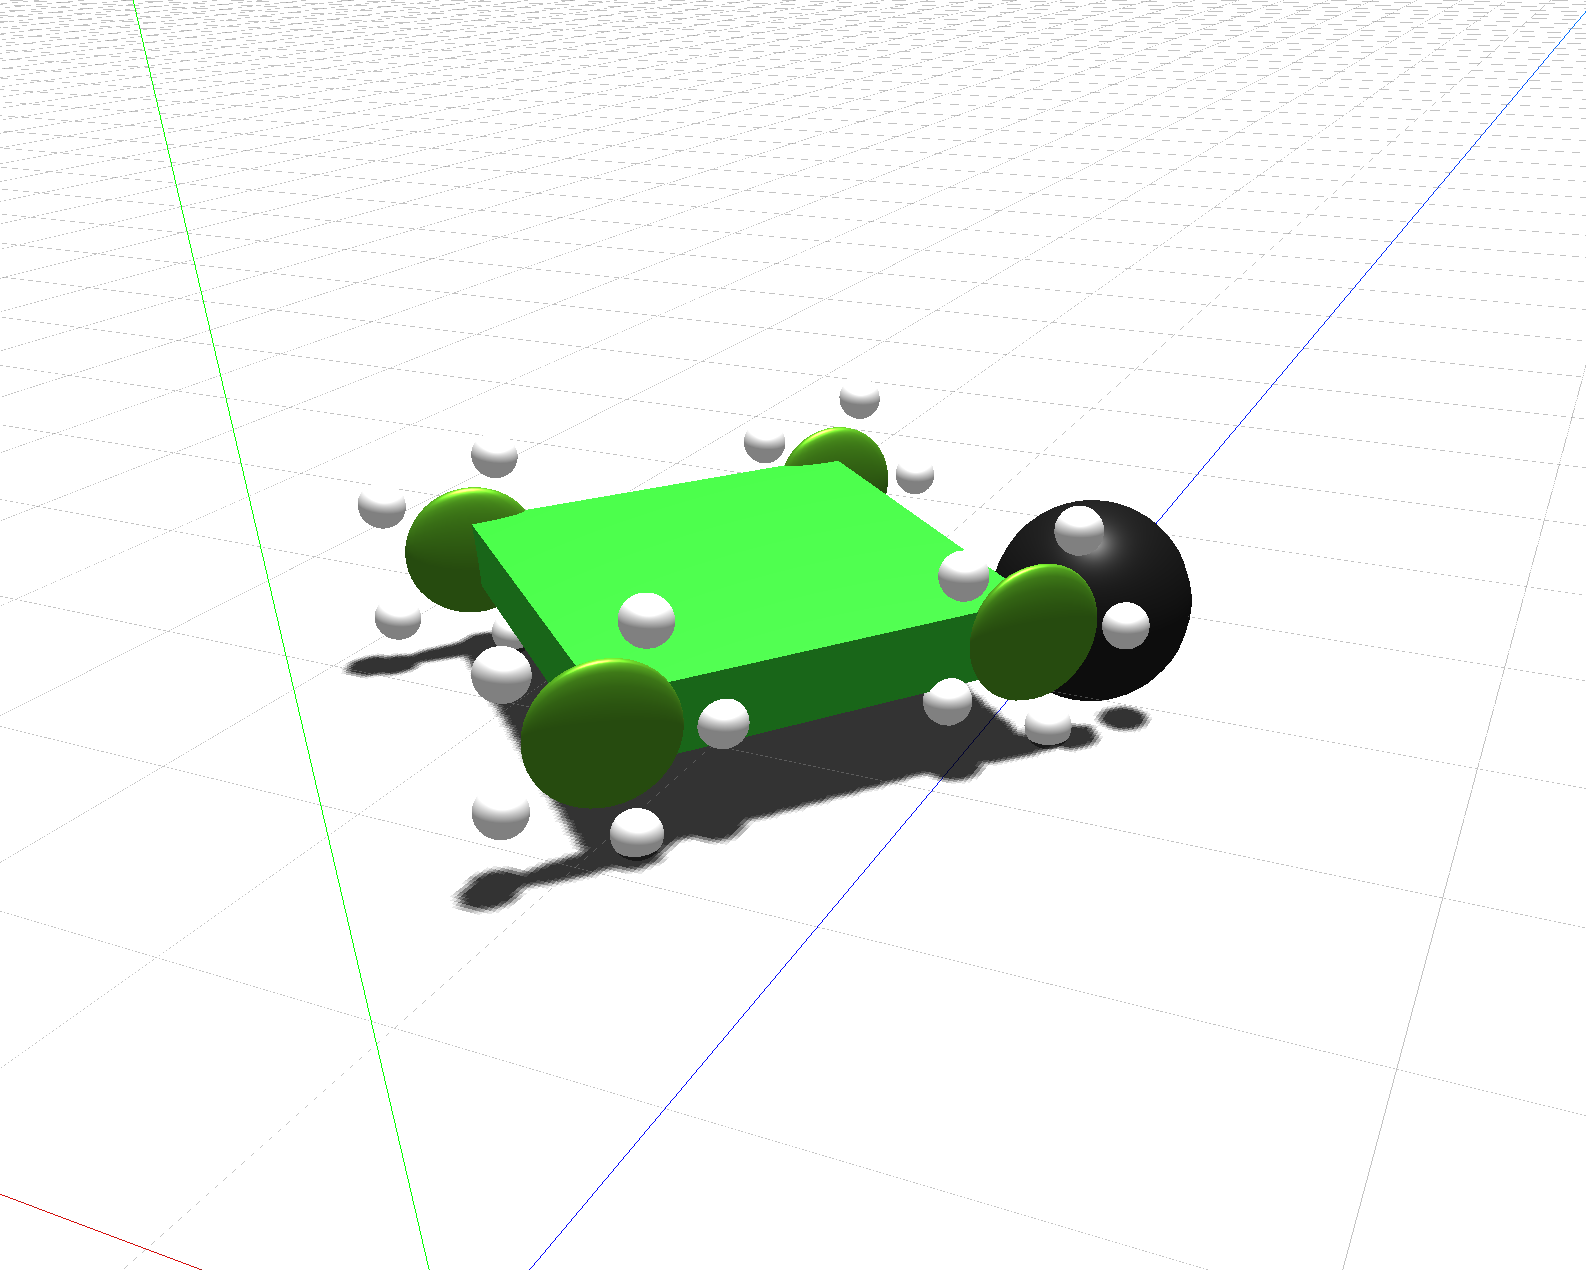
\includegraphics[width=0.4\columnwidth,valign=c]{figures/physical-simulation.png}%
        \vphantom{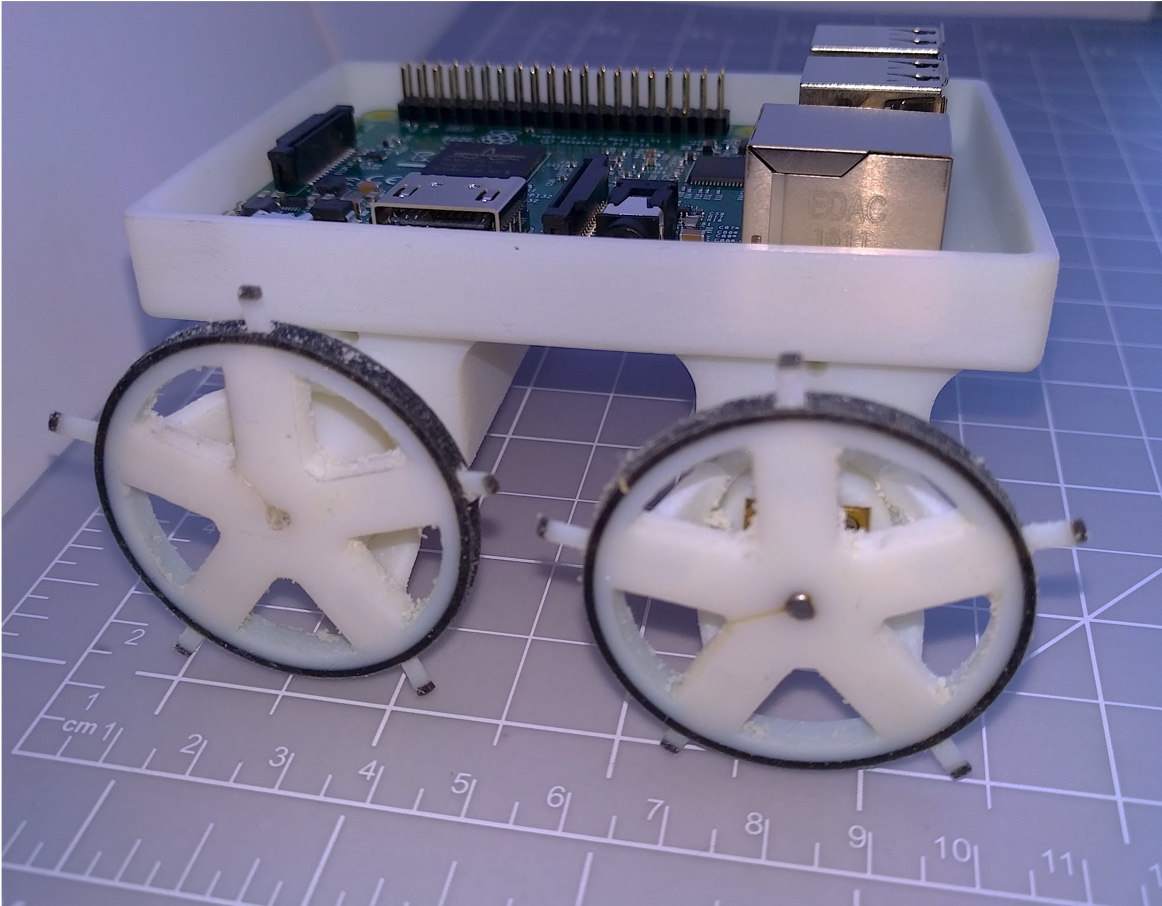
\includegraphics[width=0.4\columnwidth,valign=c]{figures/perspective-image.jpg}}%
    }\quad
    \subfloat[Prototype]{%
        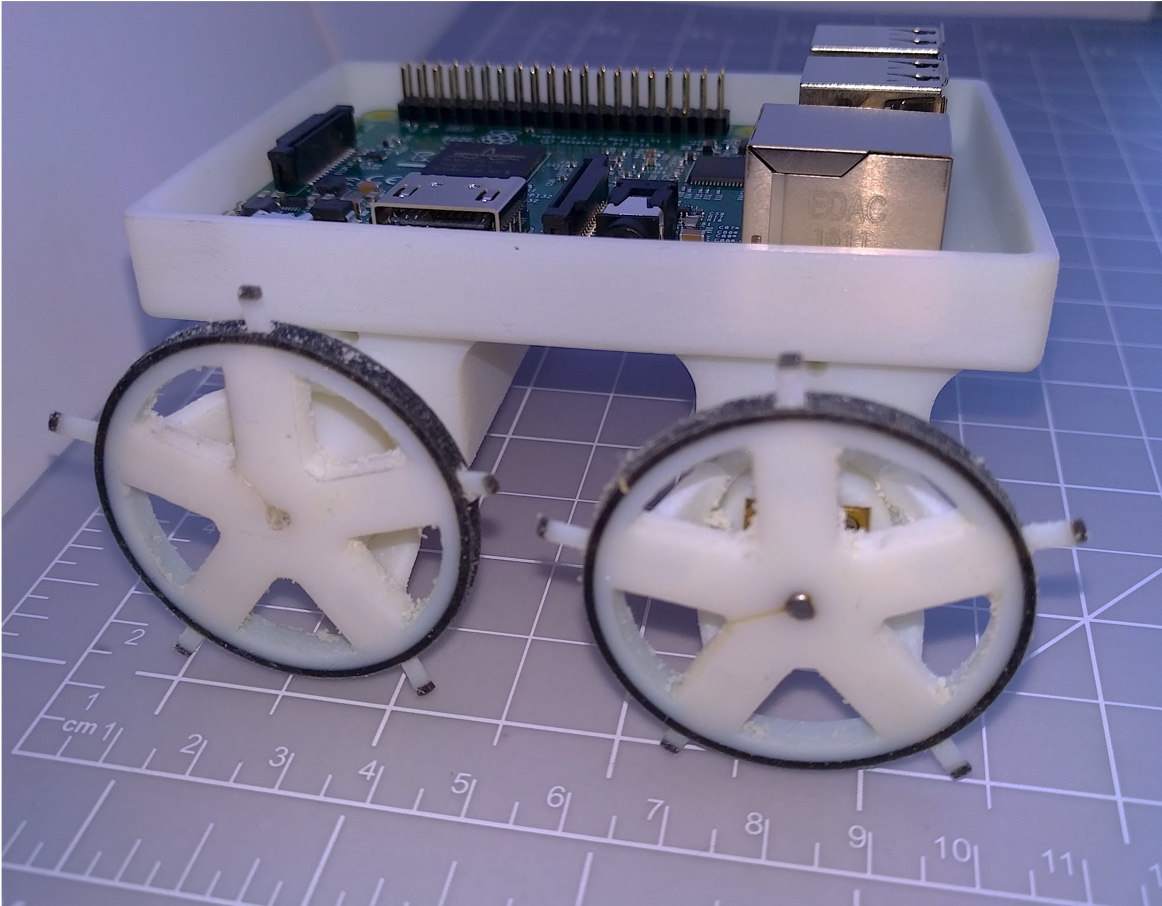
\includegraphics[width=0.4\columnwidth,valign=c]{figures/perspective-image.jpg}%
    }

    \vspace{-0.1in}

    \caption{A mobile robot with transformable wheels.}
    \label{fig:robot}

    \vspace{-0.45in}

\end{figure}

A drawback of using a transformable wheel mobile robot (or a legged-wheel robot) is that they are difficult to model.
%
Without an accurate model of the robot, it is difficult to determine when wheels should transform from normal wheels into legged-wheels.
%
Specifically, a model can calculate the \emph{expected} velocity of the robot, and we can compare this quantity to the \emph{real} velocity as measured by sensors. If these two quantities differ by some threshold amount, then the robot should infer that it is stuck or slipping (i.e., it is exhibiting poor mobility) and it should extend its wheel struts.
%
Without an accurate model of the robot kinematics, this process cannot work.


\begin{figure*}[ht]
    \centering
    \subfloat[]{%
        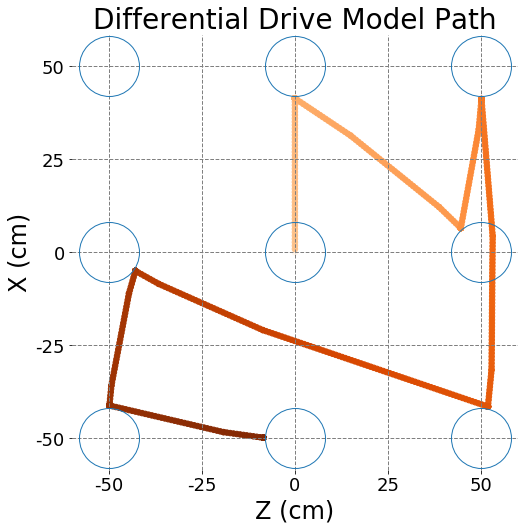
\includegraphics[height=1.6in]{figures/ddm-path.png}%
    }\hfil
    \subfloat[]{%
        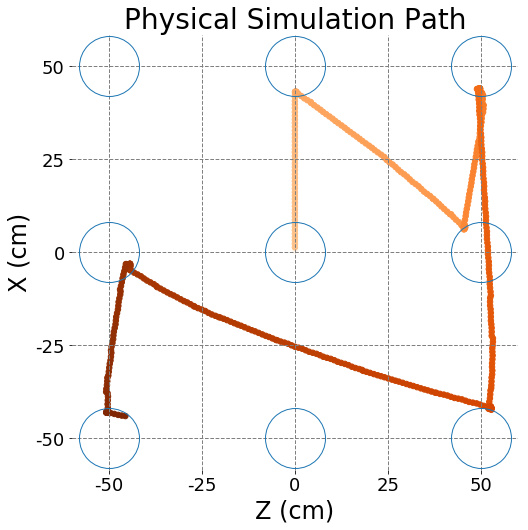
\includegraphics[height=1.6in]{figures/phy-path.png}%
    }\hfil
    \subfloat[]{%
        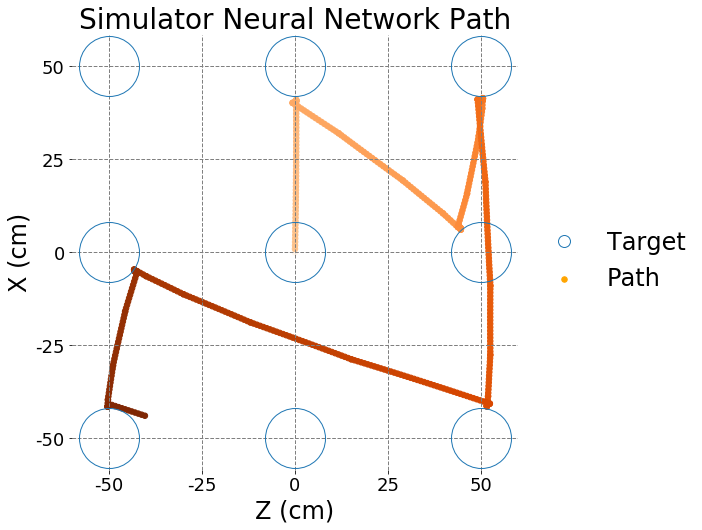
\includegraphics[height=1.6in]{figures/snn-path.png}%
    }
    %\vspace{-0.05in}
    \caption{Example paths taken by the robot (a) as predicted by the differential drive model, (b) during a physical simulation, and (c) as predicted by a trained SNN. Blue circles represent way-points that the robot is trying to reach in a pre-defined sequence. The robot moves on to its next way-point once it reaches to within 10\si{cm} of its current target way-point. Robot paths are shown in orange, and lighter shades denote earlier an earlier time in simulation (the robot starts at the origin).}
    \label{fig:paths}
    %\vspace{-0.15in}
\end{figure*}

\noindent
\textbf{Related work.}
%
In prior work, we use a differential drive model to calculate \emph{expected} velocity~\citep{Clark.2018.C.EvolvingControllersTransformable}. This process was error prone.
%
The model did not account for strut extension, wheel slippage (i.e., differing friction properties of different terrains), uneven ground, or that the wheels might rotate at a different rate than commanded.
%
In this study, we develop a simulator neural network (SNN) similar to that described by \citet{Pretorius.2014.2ICECC.ComparisonNeuralNetworks}, where they train a neural network so that control signals map to changes the pose of the robot.
%
The goal of this study is to produce an accurate model of our mobile robot. The model will have two uses: (1) to act in place of a physical simulation for optimizing control parameters and (2) to determine when the robot exhibits poor mobility and should extend struts.


\section{Training a Simulator Neural Network}

The goal of our study is to develop an SNN that can determine a new pose for our mobile robot based on the input control signals. To train the neural network, we first needed to collect training data.

\noindent
\textbf{Collecting training data.}
%
We built a physical simulation of our robot using DART~\citep{Lee.2018.JOSS.DARTDynamicAnimation}.
%
We can run the simulation with different values for the robot’s input control signals: the speeds of the left and right wheels and the strut extension amount. The simulation did not include any obstacles or uneven terrain.
%
We ran the simulation with 9012 different combinations of these input signals and collected the resulting change in position and heading.

\noindent
\textbf{Training the SNN.}
%
The SNN comprises three neural networks, one for predicting the change in the longitudinal position, one for lateral position, and one for heading.
%
We evaluated several neural network hyper-parameter combinations (i.e., architectures, optimization algorithms, learn rates, etc.). We achieved the highest accuracy on our validation data when using a network with two hidden layers, each with 20 nodes, and the L-BFGS optimizer with an adaptive learning rate.

\noindent
\textbf{Comparing the SNN model.} Figure~\ref{fig:paths} shows paths of a robot as dictated by the differential drive model, the physical simulation, and our trained neural networks.
%
As shown in the figure, compared to the kinematics model the SNN more closely resembles the actual path of the simulated robot.
%
Other example paths (using different control parameters) showed similar relative performances between the SNN and the differential drive model.
%
The SNN outperforms the differential drive model because it takes into account the wheel extensions and slippage.
%
Since the SNN takes into account these physical properties and limitations, and the real world has even more sources of noise and external influence, we expect the relative accuracy of the SNN to be even higher when these experiments are repeated with our physical device.

\noindent
\textbf{Evolving a simple controller.}
%
As the SNN is an accurate model of the physical simulation, we next attempted to use the SNN to optimize a simple controller for performing the way-point following task (as shown in Figure~\ref{fig:paths}).
% 7.5 vs .28
An advantage of using the SNN is that it is approximately 30 times faster than the physical simulation. Thus on a standard laptop, optimizing a simple finite state machine with differential evolution took only two minutes, whereas it would have taken one hour using our physical simulation.
%
An interactive visualization of the way-point following robot can be found at this address: \url{http://bit.ly/2ChVuqr}.


\noindent
\textbf{Conclusions.} We have two goals for the SNN: (1) to act in place of a physical simulation and (2) to detect poor mobility and dictate when wheel struts should extend.
%
In this study, we demonstrated goal (1) by evolving the parameters of a simple controller for way-point following.
%
As part of our ongoing studies, we will use the trained SNN to detect poor mobility when the robot is operating in an environment with obstacles and uneven terrain, and we will perform similar experiments on our real device. All code for this study can be found in this repository: \url{https://github.com/anthonyjclark/adabot-snn/}.

% \input{sections/3-discuss}
% \section{Acknowledgements}

This work was supported by


\footnotesize
\bibliographystyle{apalike}
\bibliography{refs}

\end{document}
